\documentclass[12pt]{article}

\def \projectTitle {F20DL Data Mining \& Machine Learning}
\def \projectSubtitle {Coursework 1}

\def \authorOne {Cameron McBride}
\def \authorOneID {H00160548}

\def \authorTwo{Jordan Walker}
\def \authorTwoID {H00222194}

\def \authorThree{Christopher Walsh}
\def \authorThreeID {H00122841}

%*******************************************************************************
% Geometry

\usepackage{geometry} 	% to change the page dimensions

\geometry{a4paper} 		% or letterpaper (US) or a5paper or....
\geometry{margin=1in} 	% reset margins

%%% Hyperlink Setup *************************************************************

\usepackage{hyperref} 	% for hyperlinks

\hypersetup{
	unicode=false,          % non-Latin characters in Acrobat’s bookmarks
	pdftoolbar=true,        % show Acrobat’s toolbar?
	pdfmenubar=true,        % show Acrobat’s menu?
	pdffitwindow=false,     % window fit to page when opened
	pdfstartview={FitH},    % fits the width of the page to the window
	pdftitle={\projectTitle},    % title
	pdfauthor={\authorOne,\authorTwo, \authorThree},     % author
	pdfsubject={\projectTitle},   % subject of the document
	colorlinks=true,       % false: boxed links; true: colored links
	linkcolor=blue,          % color of internal links (change box color with linkbordercolor)
	citecolor=blue,        % color of links to bibliography
	filecolor=green,      % color of file links
	urlcolor=blue           % color of external links
}

%Color Defintions *******************************************************************************

\usepackage{color} 		% to style custom colours

\definecolor{blue}{rgb}{0.22,0.25,0.70}% light blue
\definecolor{grey}{RGB}{128,128,128}% light grey

%%%*******************************************************************************
%%% ListListings

%\usepackage{courier} %% Sets font for listing as Courier.
\usepackage{listings, xcolor}
\lstset{
	tabsize = 4, %% Sets tab space width.
	showstringspaces = false, %% Prevents space marking in strings, string is defined as the text that is generally printed directly to the console.
	numbers = left, %% Displays line numbers on the left.
	commentstyle = \color{green}, %% Sets comment color.
	keywordstyle = \color{blue}, %% Sets  keyword color.
	stringstyle = \color{red}, %% Sets  string color.
	rulecolor = \color{black}, %% Sets frame color to avoid being affected by text color.
	basicstyle = \scriptsize \ttfamily , %% Sets listing font and size.
	breaklines = true, %% Enables line breaking.
	numberstyle = \tiny,
}

%*******************************************************************************
% References

\usepackage[style=numeric,backend=bibtex]{biblatex} 	% for references
\addbibresource{references.bib} % for references

%*******************************************************************************
% Images
\usepackage{graphicx}

%*******************************************************************************
% For positioning of floats.
\usepackage{float}


%*******************************************************************************
% Turn off auto paragrah indendting.
\setlength{\parindent}{0pt}

\begin{document}


\begin{titlepage}
\begin{center}
		\vspace*{3cm}
		{\Huge \color{blue}{\projectTitle}}\\[4mm]
		{\huge \color{grey}{\projectSubtitle}}\\[2cm]
		
		{\Large {\authorOne} ({\authorOneID})}\\[4mm]
		{\Large {\authorTwo} ({\authorTwoID})}\\[4mm]
		{\Large {\authorThree} ({\authorThreeID})}\\[4mm]
		
		\vspace{6cm}
		
		{\large \color{grey}{Date:}}
		{\large \today}
		
		\vspace{2cm}
		
		Link to all documents including scripts, data Files etc. can be found at: 
		\href{https://github.com/cdw2/data_mining_cw1}{https://github.com/cdw2/data\_mining\_cw1}\\
		
		{\color{grey} \footnotesize *will be public after Submission Date. }
		
		\vspace{3cm}
\end{center}
\end{titlepage}

\section{Tasks 1, 2 \& 3}

\subsection{Task 1}


The first task was to convert the CSV files into the WEKA specific Attribute-Relation File Format (ARFF) \cite{wakito2008}. To do this, we used Python to write a script ``\textbf{csv\_arff.py}'' which accepts as input a CSV file.\\

The script skips the first line of the input file to ignore the header information. Then we use Python's built-in CSV library to parse one row at a time and split the values up into a list. We take the first value of the list and convert it to a string representing the emotion. We take the second value string and split it into spaces to create an array of pixel values. From this, we create a string representing each instance, formatted to suit the .arff file and add it to a list for output. We then write out the header information to the .arff file and for each item in the output list write it to a new line in the .arff file.


\subsection{Task 2}

For this part of the coursework, we decided that it would be better to create two different scripts for the randomisation of the data we are working with throughout the course these include;

\begin{enumerate}
	\item \textbf{shuffle.py}
	\item \textbf{makeR.py}
\end{enumerate}

The \textbf{shuffle.py} program works on any .arff and is used to swap entries in the data of that particular file. By doing this, it results in no loss of any data, however, the position of each data entry changes which removes any bias. I.e. if you trained the model one after the other in the original file and the file which was created in such a manner that the properties of the predecessor data entry affected the following entry then this is the bias which will be removed by shuffle.py.\\

\textbf{makeR.py} works by making one new file from all the data entries from each fer2018EmotionX arff file combining them and creating a reliable dataset where there are equal amounts of entries from each emotion file. This is achieved by allowing the user to select the data size they want and checking that is a modulo of 7. This produces a robust dataset where there could perhaps be issues with more entries of one emotion than another which may affect the learning of the model. Using this with the shuffle in our opinion was the best practice for making good data samples that are randomised.\\

By shuffling and taking random samples of the data files, we can say that we serve the idea of reducing variance and making sure that the data model stays general and we reduce the risk of overfitting. By taking a fair amount of data entries from each EmotionX file, we can say that our training, testing and validation are more representative of the data-set as a whole.\\

\newpage

\subsection{Task 3}

Cameron Explain\\

For our implementation we increased the “heap” size of \textit{WEKA} to 4GB allowing us to use the whole data set rather than just a smaller collection of the data entries.\\ 


\section{Tasks 4, 5, 6 and 7}

\subsection{Task 4 - Classification: Performance of the Nearest Neighbour Algorithm on the given data set}

After we had reduced our number of attributes we also normalised the pixel values using the \textit{WEKA} filter. The motivation for this is that the pixel values can vary over a wide range (0-255) and the K-nearest neighbour algorithm works by looking at the nearness of other data points typically based on euclidean distance. Therefore normalization allows for more accurate classification by bringing the values into a smaller range (0-1).\\

During Task 3 our solution to the task allowed us to reduce the “noise” of the images. Thus because of this we did not need to add another \textit{WEKA} filter as we essentially created our own implementation of a “noise reduction” filter.\\ 

\begin{figure}[H]
	\centering
	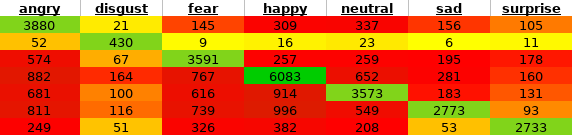
\includegraphics[width=0.7\linewidth]{images/heatmap}
	\caption{Confusion Matrix}
	\label{fig:heatmap}
\end{figure}

\begin{figure}[H]
	\centering
	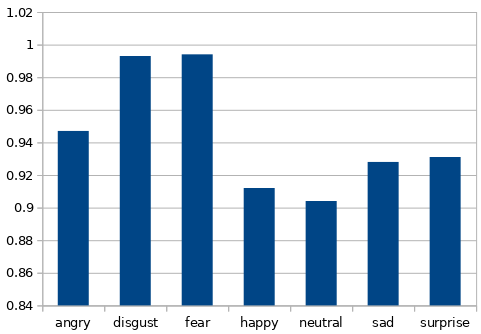
\includegraphics[width=0.5\linewidth]{images/roc_graph}
	\caption{ROC Bargraph}
	\label{fig:roc_graph}
\end{figure}


Above you can see the results of our first run of the nearest neighbour with k =3.\\

\subsection{Task 5 - Deeper analysis of the data }

For this task we amended our ``\textbf{csv\_arff.py}'' script to allow the conversion of the individual emotion files to only have the correct emotion name and “other”. This allowed them to be loaded into \textit{WEKA} and have correlation tests performed on them.\\

Using the \textit{WEKA} select attribute tab with the Correlation Attribute Evaluator selected and the Ranker search method. Here are the values for the 10 most relevant attributes for each emotion file.\\

\begin{figure}[H]
	\centering
	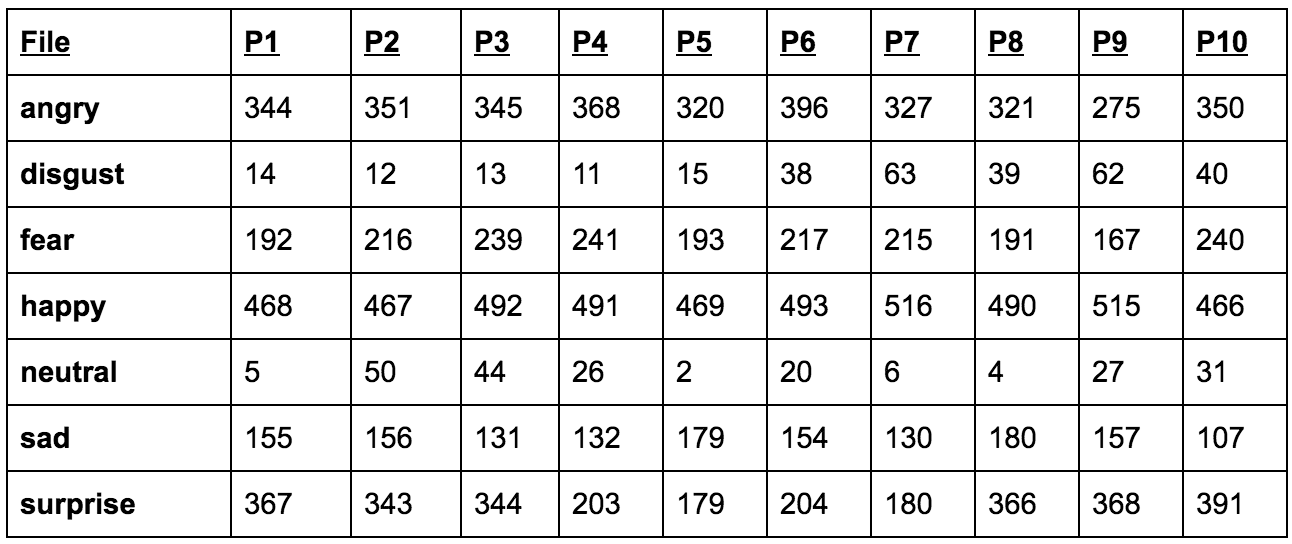
\includegraphics[width=0.7\linewidth]{images/task5_results}
	\caption{Task 5 : Top 10 pixel correlation values}
	\label{fig:task5_results}
\end{figure}

\begin{figure}[H]
	\centering
	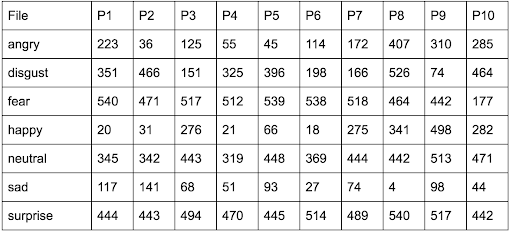
\includegraphics[width=0.7\linewidth]{images/task5_results_2}
	\caption{Task 5 : Bottom 10 pixel correlation values}
	\label{fig:task5_results_2}
\end{figure}

\textbf{Note:} Our filter reduced the pixel range from 48 x 48(2304)  to 24 x 24 (576).

\subsection{Task 6 - Improve the classification}

For part 6 we wrote a script ``\textbf{extract\_pixels.py}'', to extract specific pixel values from each file and assemble them into a whole dataset.\\ 

We used the data gathered in part5 to extract the pixels for the top 2, 5 and 10 class attributes. This resulted in datasets with 14, 35, and 70 pixel attributes.\\

We imported these into \textit{WEKA}, normalised the pixel values and ran the IBK Nearest Neighbour classifier again with K set to 3.\\ 

\subsection{Task 7 - Make Conclusions}

\vspace{4mm}

\textbf{Which emotions are harder to recognise?}\\

The happy and neutral emotions were hardest to recognise.\\

\noindent\textbf{Which emotions are most easily confused?}\\

Angry happy and neutral were the most easily confused.\\

\noindent\textbf{Which attributes (fields) are more reliable and which are less reliable in classification of emotions?}\\

See figures \ref{fig:task5_results} and \ref{fig:task5_results_2} for the top 10 best and worst attributes for the classification of emotions.\\

\noindent\textbf{What was the purpose of Tasks 5 and 6?}\\

The purpose of tasks 5 and 6 was to perform attribute selection on our data. The reason behind attribute selection is to reduce the dimensionality of the data. This reduces the training time of the models and can increase accuracy by reducing noise in the data, reducing overfitting and avoiding spurious correlations.\cite{sain2010}\\

\textbf{What would happen if the data sets you used in Tasks 4, 5 and 6 were not randomised?}\\

The resulting classifier would be poorly trained as the data would be grouped by class, so you would not get a good representative sample of the data between the training and test data.\\

\textbf{What would happen if there is cross-correlation between the non-class attributes? }\\

If there was a cross correlation between each image there would be no way to classify which emotion is which. If we imagine that the “strongest” pixels were always the same or close then the classifier would experience a high error rate as each entry regardless of emotion would share the same values that make them distinguishable.\\ 


\textbf{Other methods we could of tried? }\\

Two possible methods appear when thinking about image classification:

\begin{enumerate}
	\item Using another model
	\item Using different data
\end{enumerate}

When working with any data mining set it is apparent that there are many different models that could be used to extract the data you are looking for. For example in this project we could of implemented a Neural Network where we feed the network line by line training data and then have that line “classed” as a certain emotion. Afterwards we could insert our fer2018 datafiles and achieve a different type of classifier for the images.\\

The second aspect we could of tested would be to use different data i.e. instead of pixel data we could of used ratio data where we feed the classifier attributes such as the width between eyebrows, the height between the left eye and the left lip etc.\\ 

In general practice we could assume these attributes may give similar or even greater results for classifying emotions from images.\\

\textbf{Would there be more accuracy by using a Neural Network for this type of project?}\\

In 2015 there was an experiment done trying to determine if combining a Neural Network and K- Nearest Neighbour models would produce better classification results. The experiment was run on ratios as attributes rather than pixel values as our own. However, during this experiment the Neural Network showed a better classification average of 0.95\%. \cite{hai_2015}.\\

We can assume we had implemented a Neural Network rather than K-Nearest Neighbour we could assume there would be an increase of accuracy in our classification.\\


\section{Masters Question (For our own understanding)}

\subsection{The effects on Nearest Neighbour of varying numbers of neighbours}

To test the classification on changing the K value of the Nearest Neighbour algorithm we ran tests on K set to one, two and the original testing requirement of three. As seen in figures \ref{fig:masters1} and \ref{fig:masters2}, we observe that when the K value is changed we see a very dramatic decrease in the correctly classified instances and a sharp increase in the incorrectly classified images.\\

\begin{figure}[H]
	\centering
	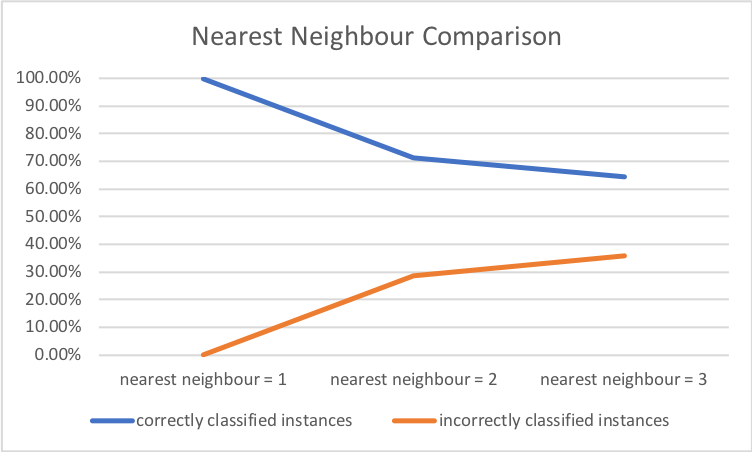
\includegraphics[width=0.7\linewidth]{images/masters1}
	\caption{Masters: Nearest Neighbour Comparison}
	\label{fig:masters1}
\end{figure}

\begin{figure}[H]
	\centering
	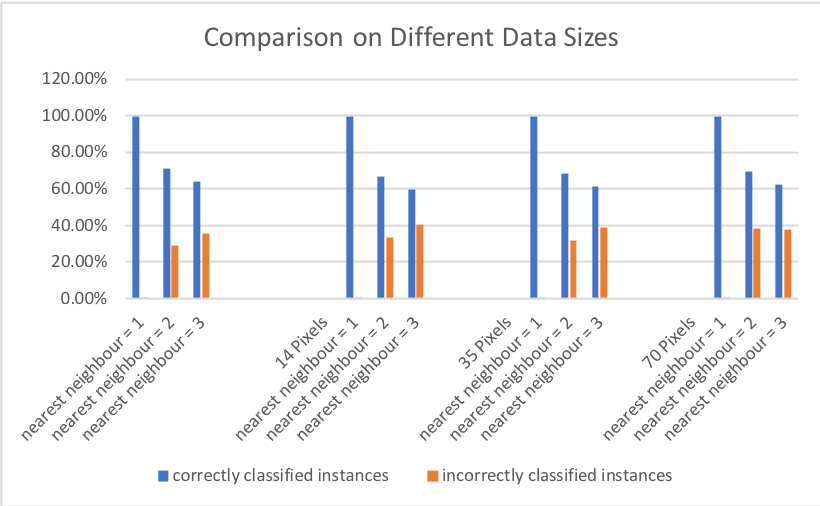
\includegraphics[width=0.7\linewidth]{images/masters2}
	\caption{Comparison running IBK on different numbers of attributes.}
	\label{fig:masters2}
\end{figure}

We can establish that the data size doesn't matter. Because of the type of data (numeric) grouping nearest neighbour becomes a lot more difficult. Because of that the noise of the image itself is increased.\\

Hence the vast reduction in correctly classified instances and the increase in incorrectly classified instances.\\

\newpage
\printbibliography

\newpage
\section{Appendices}

\subsection{Task 4 Screen-shot}

\begin{figure}[H]
	\centering
	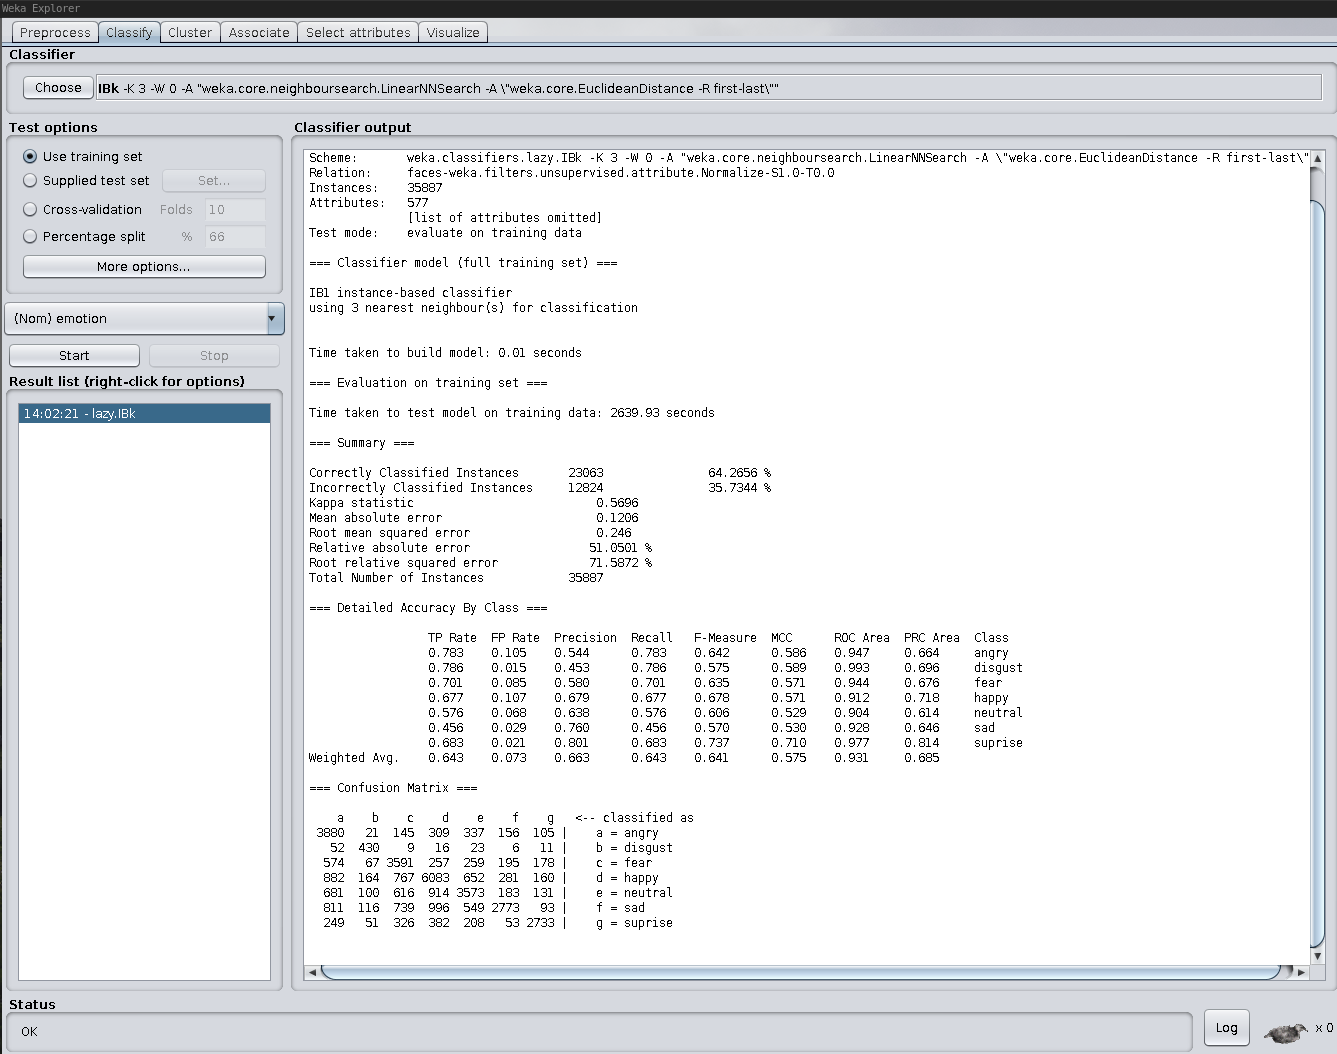
\includegraphics[width=1\linewidth]{images/task4_1}
	\caption{Task 4: Reduced Dataset, Normalised NN3}
	\label{fig:task4_1}
\end{figure}

\subsection{Task 6 Screen-shots}

\begin{figure}[H]
	\centering
	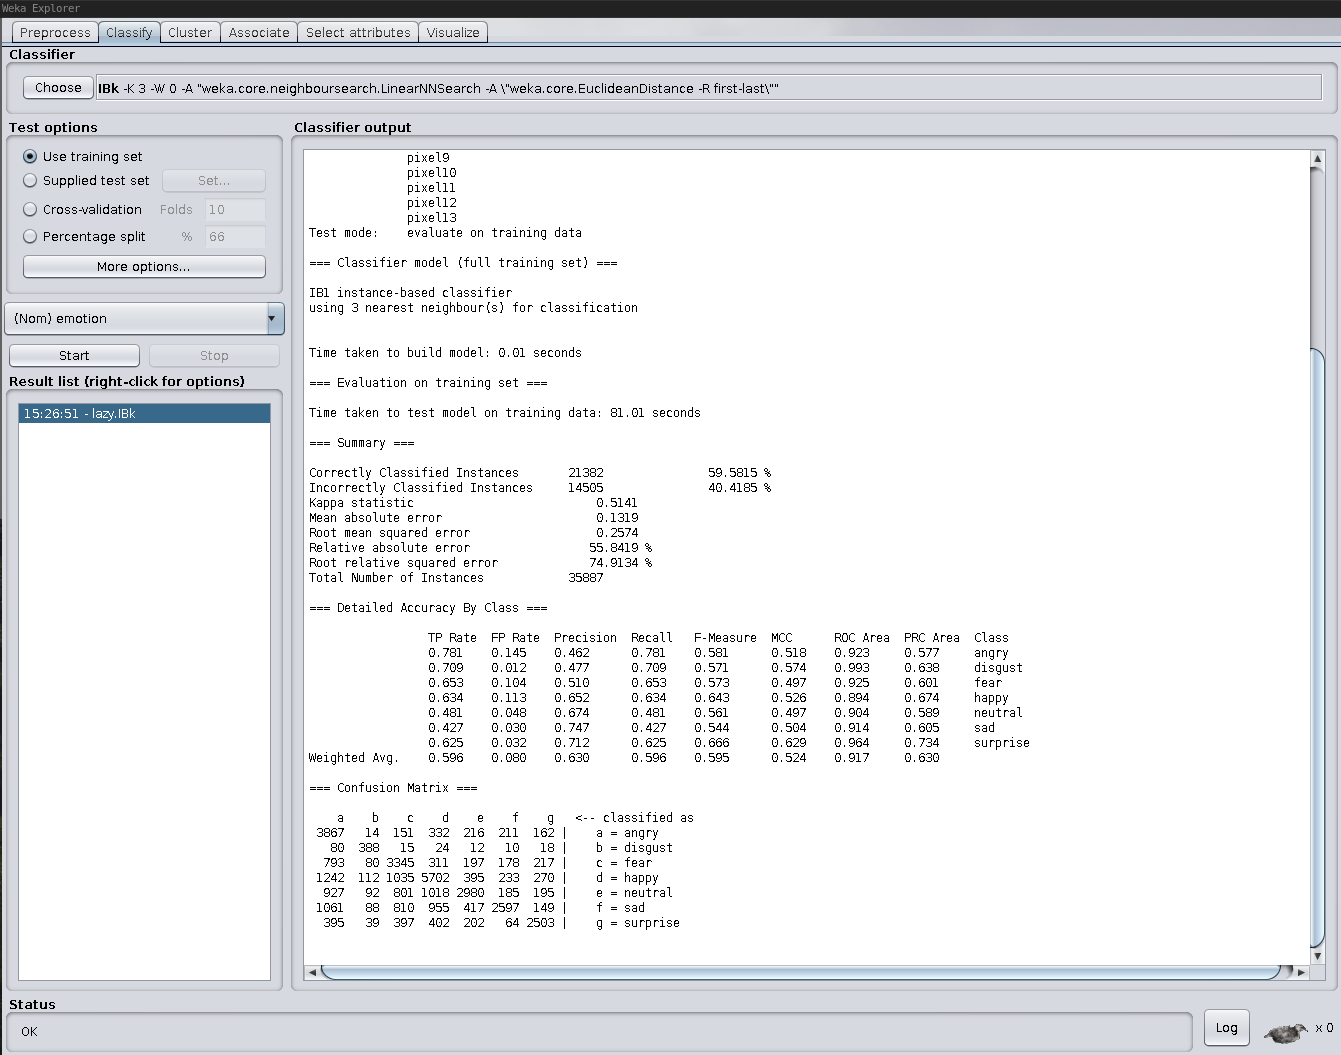
\includegraphics[width=1\linewidth]{images/14_pixels}
	\caption{Task 6: 14 Pixels}
	\label{fig:task6_1}
\end{figure}

\begin{figure}[H]
	\centering
	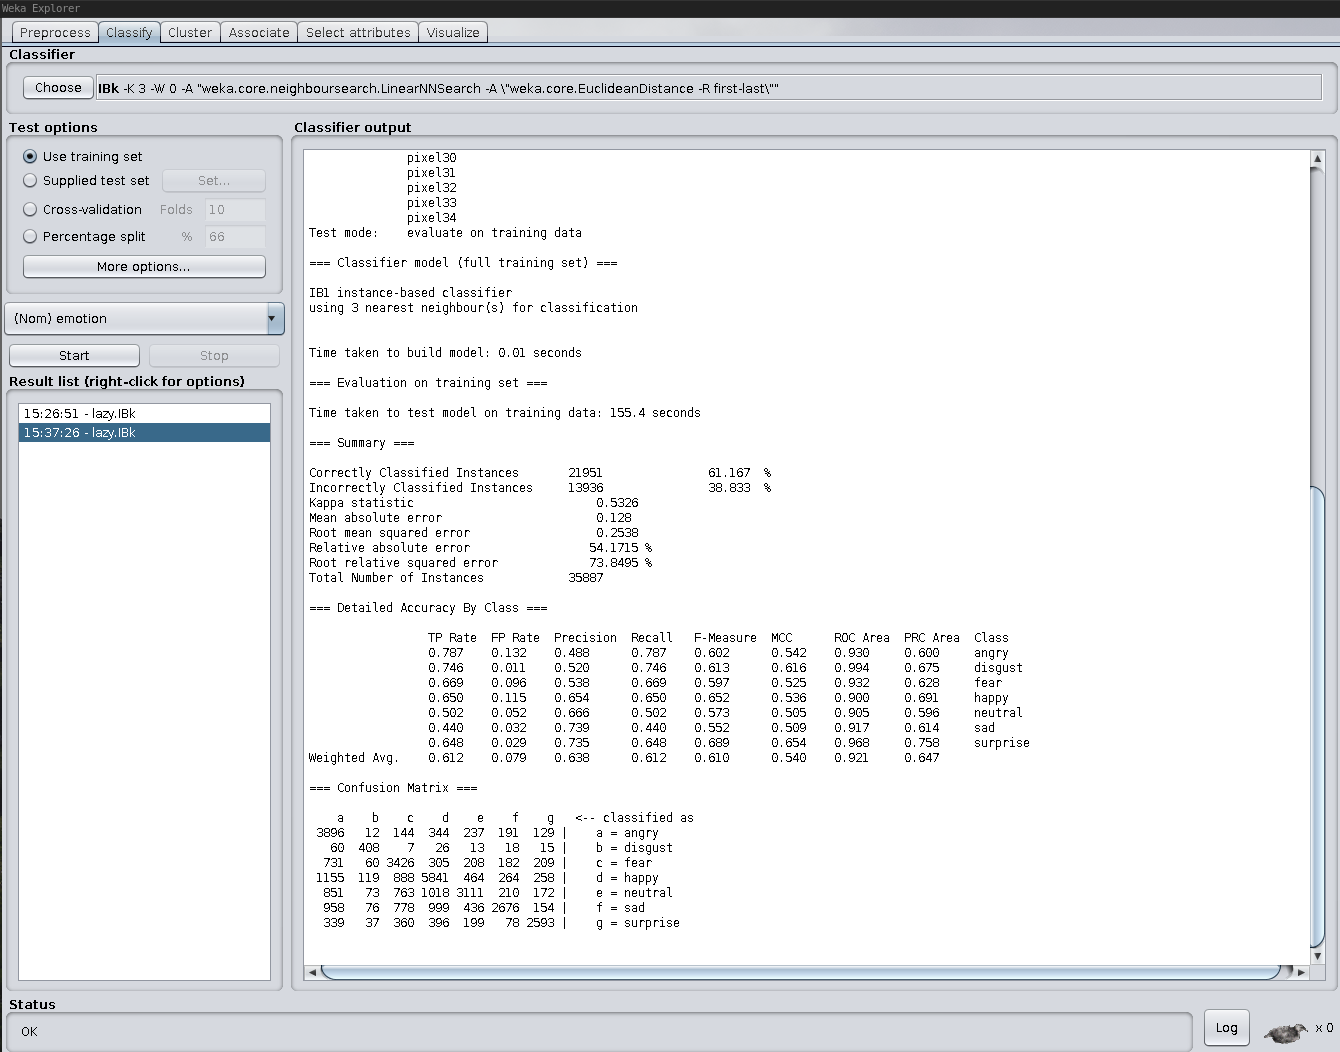
\includegraphics[width=1\linewidth]{images/35_pixels}
	\caption{Task 6: 35 Pixels}
	\label{fig:task6_2}
\end{figure}

\begin{figure}[H]
	\centering
	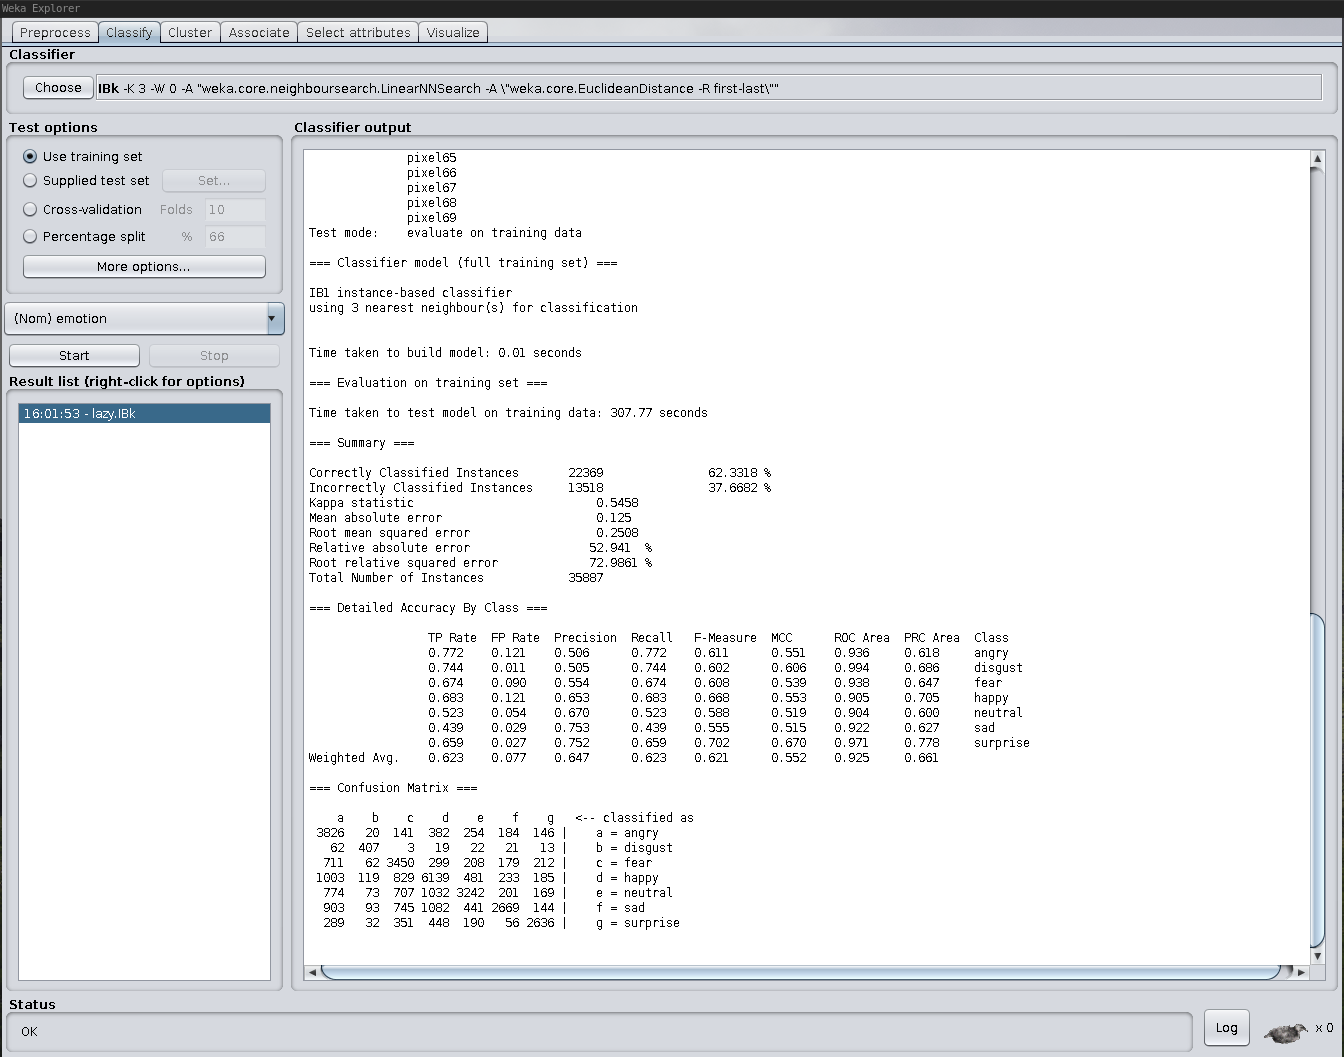
\includegraphics[width=1\linewidth]{images/70_pixels}
	\caption{Task 6: 70 Pixels}
	\label{fig:task6_3}
\end{figure}
	
\end{document}

